\documentclass[a4paper,12pt]{article}
\usepackage[lmargin=1cm,rmargin=1cm,tmargin=1cm,bmargin=1.5cm]{geometry}
 % \usepackage[utf-8]{inputenc} (si lo pones tienes problemas y la verdad no se por que . 
\usepackage[spanish]{babel}%para que te aparezca capitulo 1 en vez de chapter 1
\usepackage{amsmath}
\usepackage{amsfonts}
\usepackage{amssymb}
\usepackage{float} % Este sive para usa el [H] en el begin figure
\parindent=0mm %con esto elimino la sangría 
\usepackage{graphicx}
\usepackage{caption} % Necesario para poner caption
\usepackage{subcaption} % Necesario para las subfiguras 

\usepackage{circuitikz} %este es el paquete para crear circuitos electricos 
\usepackage{siunitx} %este paquete es para las unidades de medida

\newtheorem{preg}{Pregunta} %este es para las preguntas 

\begin{document}

\begin{itemize}
\item Nombre : Juan Alonso Alcalá Lujan 
\item Código : 20172226A 
\end{itemize}

% PREGUNTA NUMERO 1 
\begin{preg}
¿Cuáles son las partes principales de un osciloscopio de rayos catódicos (analógico) ? 
\end{preg}

Los osciloscopios analógicos tienen un tubo de rayos catódicos que consta de 3 partes fundamentales encerradas en un tubo de vidrio y con un vació elevado .
\begin{itemize}
\item Cañon de electrones
\item Dispositivo de desviación de electrones
\item Pantalla
\end{itemize}

\begin{preg}
Indique en un diagrama de bloques la estructura de 
\begin{itemize}
\item Un osciloscopio analógico
\item Un osciloscopio digital
\end{itemize}
\end{preg}


\begin{figure}[H]
     \centering
     \begin{subfigure}[b]{0.7\textwidth}
         \centering
         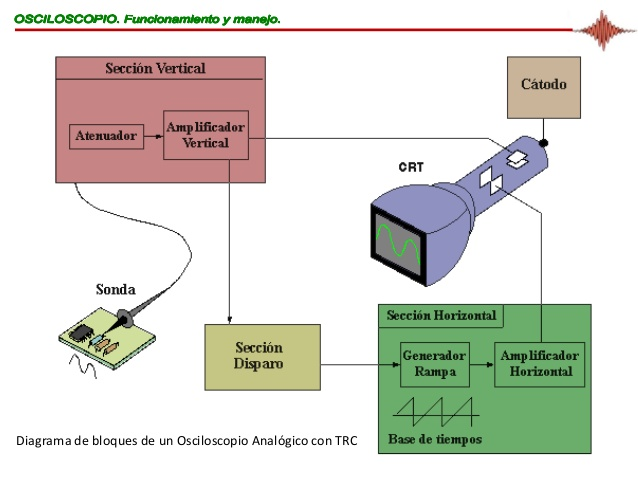
\includegraphics[width=\textwidth]{bloque_analogico.jpg}
         \caption{Analógico}
     \end{subfigure}
     \hfill
     \begin{subfigure}[b]{0.6\textwidth}
         \centering
         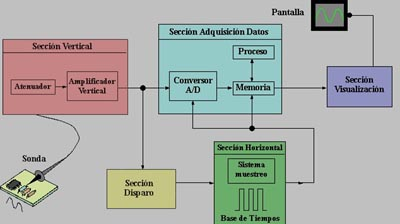
\includegraphics[width=\textwidth]{bloque_digital.jpg}
         \caption{Digital}
     \end{subfigure}
\end{figure}



\begin{preg}
¿Cómo es la señal de barrido de tiempos y en qué se utiliza?
\end{preg}

La función de este es conseguir que la tensión aplicada (de medición) aparezca en la pantalla como función del tiempo . La pantalla muestra un sistema de coordenadas que esta formado por el eje vertical ( donde se representa la medida de voltajes ) y el eje horizontal ( donde se representa los tiempos ) . El circuito de base de tiempos lo que hace es que el punto luminoso se desplace periódicamente con una velocidad cte para luego volver a la posición original . Ese proceso se repite en intervalos de tiempo para poder observar la medida de voltaje con el tiempo . (\textbf{He allí su utilidad}) . Y para conseguir eso el circuito de base de tiempo debe proporcionar a las placas horizontales una tensión variable en especifico una \textbf{Tensión de Diente de Sierra} .   



\begin{preg}
Explique cómo se forma la imagen de una señal de voltaje alterno en la pantalla de osciloscopio analógico . 
\end{preg}


Hay dos pares de placas que reciben tensiones . Las horizontales se les aplica una tensión generada internamente en forma de diente de sierra . Y las verticales se les aplica la señal que queremos estudiar . La combinación de estas desvía los electrones emitidos por la fuente hacia la pantalla . La pantalla es de un material fosforescente que emite luz en los lugares donde el electrón colisiona . Estas dos tensiones en conjunto con el disparo de electrones proyecta una imagen continua del voltaje que queremos medir .  


\begin{preg}
Explique la función de los controles \textbf{trigger} y \textbf{hold} del osciloscopio.
\end{preg}



\begin{description}
\item[Trigger:] Hace que la onda sea estacionaria . 
\item[HOLD:]Sólo en osciloscopios digitales.  Congela la imagen . Cuando se vuelve a pulsar la imagen se descongela . Cada canal se puede congelar de forma independiente. 
\end{description}



\begin{preg}
Diferencie el termino impedancia de resistencia; defina reactancia capacitiva y reactancia inductiva. 
\end{preg}


\begin{itemize}
\item La \textbf{resistencia} es una medida de oposición al paso de corriente por un resistor . La \textbf{impedancia} extiende el concepto pero para elementos de circuitos de corriente alterna (CA) . Estos poseen magnitud y fase que a diferencia de la resistencia solo tiene magnitud . 
\item La \textbf{Reactancia Capacitiva} es una medida de oposición al paso de corriente alterna . La corriente no pasa por el capacitador realmente pero si tiene una reacción contraria a este . Por causas de la naturaleza del condensador se llama reactancia capacitiva .
\item La \textbf{Reactancia Inductiva} es una medida de oposición a cambios de intensidad de corriente . Este a diferencia de otras resistencias se opone a cambios en la intensidad de corriente y no a la corriente misma que pasa por el .  
\end{itemize}



\begin{preg}
Cuál es el significado físico del valor eficaz de corriente
\end{preg}

El significado físico del valor eficaz es designar el valor de un corriente rigurosamente constante que al circular sobre una determinada resistencia ohmica produciría los mismos efectos caloríficos que dicha corriente variable . De este modo , se establece un paralelismo entre cualquier tipo de corriente variable y la corriente continua que simplifica los cálculos con esta ultima . 



\begin{preg}
Calcule el valor eficaz para distintas señales: sinodal y cuadrada
\end{preg}

\begin{itemize}
\item Sinodal : En este caso tenemos una función del tipo $ y = A_1sin(2\pi ft)$ con $ f = \frac{1}{T}$
\begin{figure}[H]
\centering
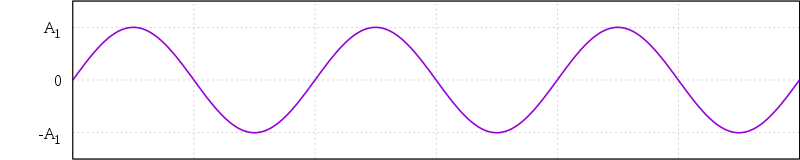
\includegraphics[width=0.5\textwidth]{Wave_sine.png}
\end{figure}
\begin{align*}
 \overline{y} &= \sqrt[2]{\dfrac{1}{T}\int_0^T y^2 dt    } \\
 \overline{y} &= \sqrt[2]{\dfrac{1}{T}A_1^2\int_0^T sin^2\left(\dfrac{2\pi t}{T}\right) dt } \\
 \intertext{Operando se obtiene}
 \overline{y} &= \dfrac{A_1}{\sqrt{2}}
\end{align*}	

\item Cuadrada : En este caso tenemos una función del tipo : 
\begin{figure}[H]
\centering
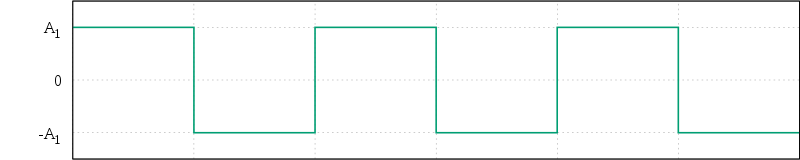
\includegraphics[width=0.5\textwidth]{Wave_square.png}
\end{figure}
\begin{align*}
 \overline{y} &= \sqrt[2]{\dfrac{1}{T}\int_0^T y^2 dt    } \\
 \overline{y} &= \sqrt[2]{\dfrac{1}{T}A_1^2\int_0^T 1 dt } \\
 \intertext{Operando se obtiene}
 \overline{y} &= A_1
\end{align*}	

\end{itemize}




\begin{preg}
En un circuito $RC$ serie como el de la siguiente figura ¿por qué se produce desfasaje entre el voltaje en el condensador y el voltaje de entrada ? Establezca la ecuación del circuito . Busque la expresión para calcular el desfasaje . 
\end{preg}

\begin{figure}[H]
\begin{center}
\begin{circuitikz}[american]
\draw (0,4) to[sV=$V$,a= 5$V_p$] (0,0) to[] (4,0) to[capacitor,a=\SI{200}{\nano\farad},l=$Z_2 $] (4,4)
 to [R, a=\SI{1}{\kilo\ohm} , l= $Z_1$] (0,4);
\end{circuitikz} 
\end{center}
\caption{circuito1}
\end{figure}

\begin{itemize}
\item El desfasaje se explica debido a la naturaleza de capacitador . Que reacciona ante los cambios bruscos de variación de voltaje . Es decir que cuando el voltaje en la fuente de poder tiene cambios el capacitador reacciona haciendo disminuir ese voltaje que quiere ofrecer la fuente de poder . Por tanto se da un desfasaje que en el máximo de la fuente de poder no concuerda con la del capacitador en el tiempo .  

\item Aplicando la segunda ley de kirchoff es fácil ver que la ecuación del circuito es :  
\begin{equation*}
 RC\dfrac{dv}{dt} + v = 5V_psin(wt) 
\end{equation*}
Donde "$v$'' es el voltaje del capacitador "$w$'' es la frecuencia de la fuente de poder \\


\item Por otro lado tenemos $Z_eq = Z_1 + Z_2 = R - j\frac{1}{wC}$ . Y pasando al dominio de frecuencia y resolviendo alli obtenemos los siguientes desfasajes 

\begin{itemize}
\item desfasaje del resistor = $ tan^{-1}(-wRC)$
\item desfasaje del capacitador = $ tan^{-1}(\dfrac{1}{wRC})$
\end{itemize}
Estos desfasajes recuerda son respecto a la fuente de poder .

\end{itemize}








\end{document}
